\chapter[Final Presentation]{Complex Population Health Challenges}
\section{Building meaningful engagement with stakeholders}

This presentation was delivered at the Senior Management Team meeting, Dorset Public Health 28 October 2015: 1330 -- 1500. The meeting was attended by the Senior Management Team and Debbie Ward, CEO of Dorset County Council.

\begin{figure}[htbp]
\centering
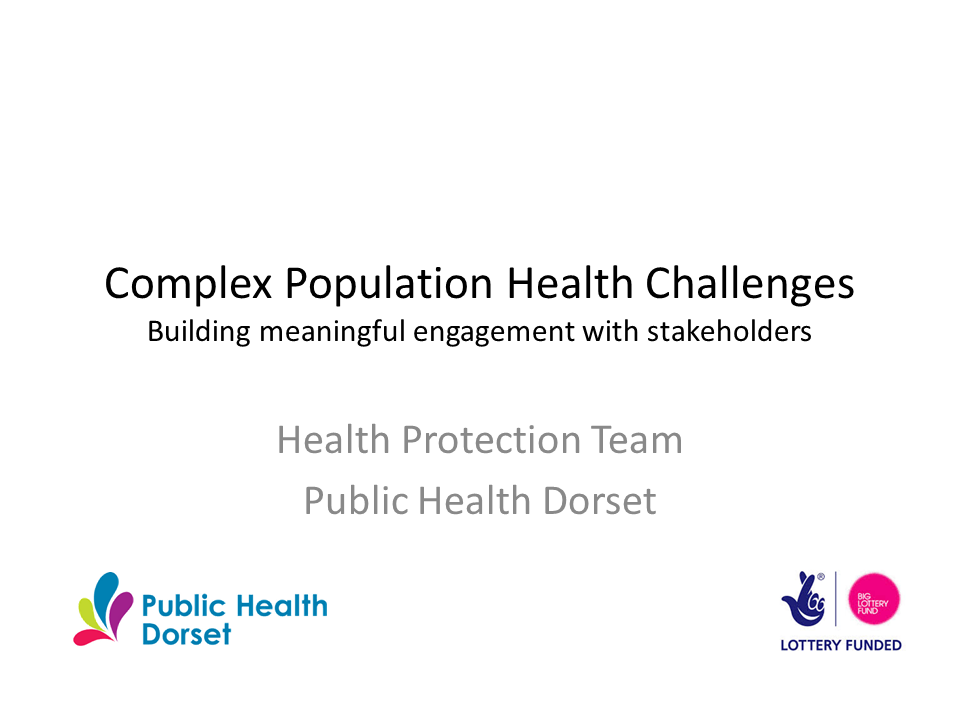
\includegraphics{img/cem1.png}
\caption[Population Health Challenges Are Complex]{Contemporary population health challenges are complex. They are complex in the sense that almost any public health intervention made today will have unintended consequences -- i.e. we can't easily predict how it will work out. Unfortunately, traditional public health since the time of John Snow makes interventions as if linear cause and effect were the rule of the day: remove pump handle, stop the cholera outbreak. 
If only life were so straight forward today! This two year research effort, now coming to a close, has identified and documented two approaches to developing more meaningful engagements with stakeholders on complex population health challenges that lie ahead of us. However, this research project didn't start out to do this.
}
\end{figure}

\begin{figure}[htbp]
\centering
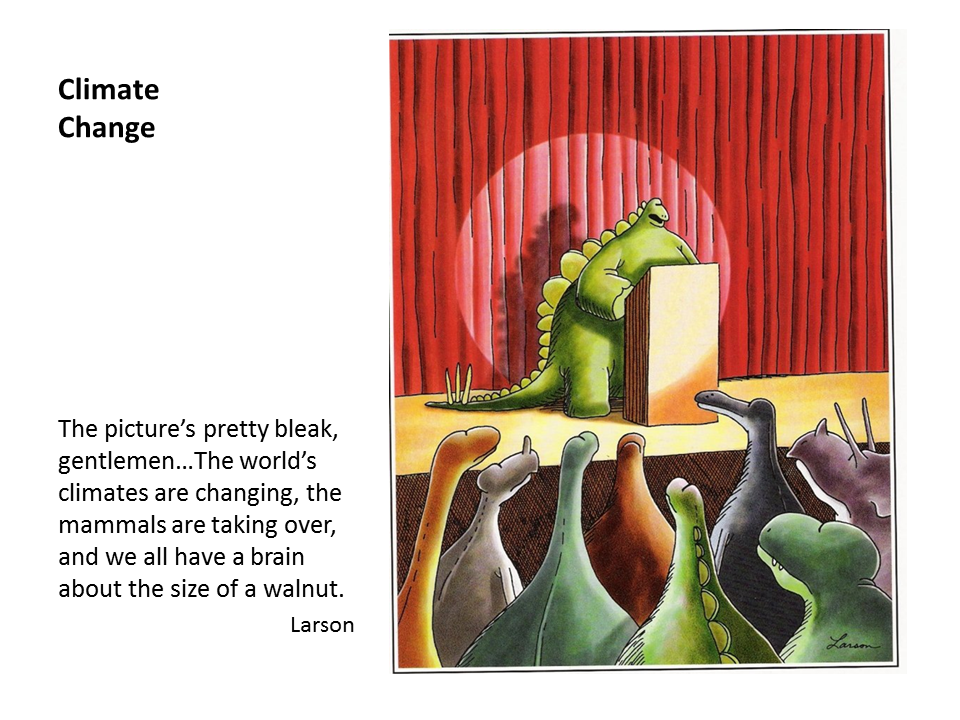
\includegraphics{img/cem2.png}
\caption[Evolution of Project Thinking]{The research project started out to examine ``the potential health impacts facing older people in West Dorset from the onset of climate change in 2030''. The title alone was enough to leave most of our stakeholders looking for a way out the engagement. Climate change is a complex challenge. The `ageing' of our population is a complex challenge. Climate change, ageing, and health impacts -- is very complex. And we haven't even begun to talk about formulating and implementing public health interventions. We might know a lot more that John Snow ever knew, but it's not enough. We need new approaches to understanding and communicating complexity with out stakeholders.}
\end{figure}

\begin{figure}[htbp]
\centering
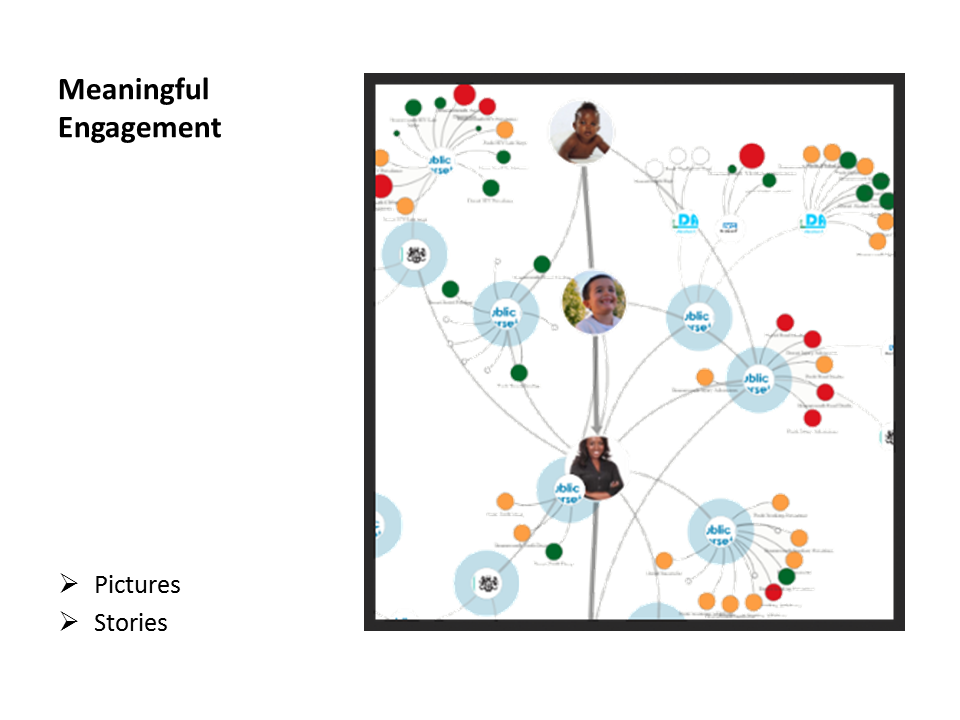
\includegraphics{img/cem3.png}
\caption[Meaningful Engagement]{Meaningful engagement means being able to have an informed discussion about important population health issues, where there is some hope of developing a `shared understanding' of the challenges we face. It doesn't even mean agreeing on a way forward -- it just means being able to have an informed discussion. Something that is now very often not possible. If public health professionals and scientists are to engage policy makers in a meaningful discussion, we need to change our approach. If public health professionals and scientists are to bring the public along with the development of new evidence and new interventions, we need to change our approach. We believe that an approach that includes pictures and stories has potential to improve engagement.}
\end{figure}

\begin{figure}[htbp]
\centering
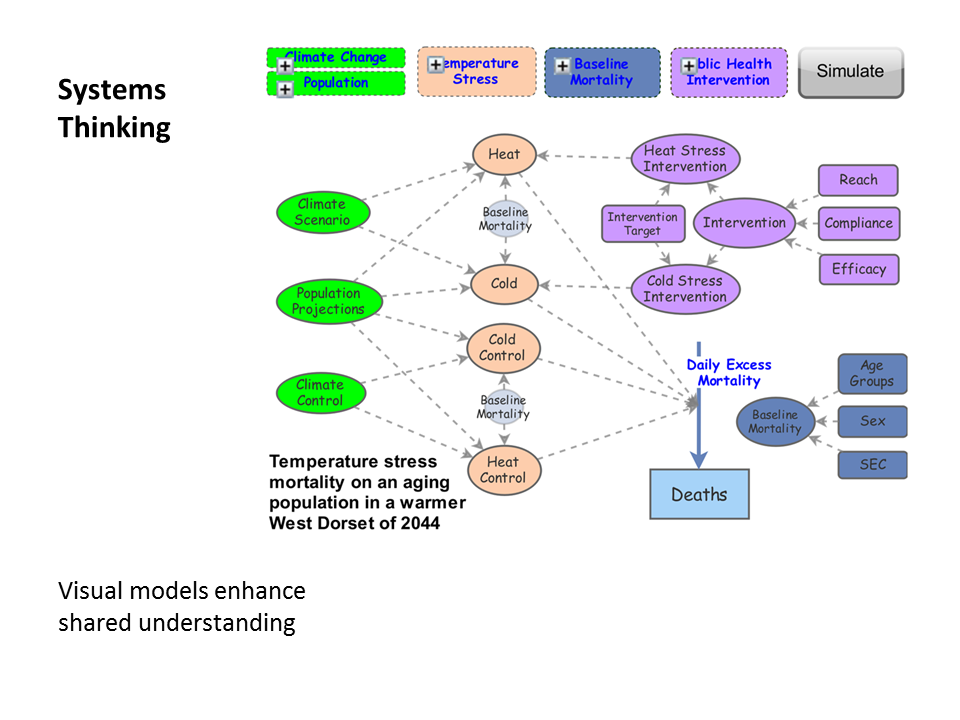
\includegraphics{img/cem4.png}
\caption[The Systems Thinking Perspective]{This systems picture of the ``climate impacts on the health of older people'' illustrates this grand challenge of complexity. It combines ONS population projections and Met Office climate scenarios to estimate excess mortality from heat and cold stress thirty years from now. This system picture indicates the deaths that will occur due to the `daily excess mortality' above baseline mortality. The public health interventions that may be possible can be modelled using only three elements that define all possible interventions: the population reach of the intervention, the population compliance with the intervention and the efficacy of proposed interventions. The systems tools that allow for this visualisation, also provide online story telling capability.}
\end{figure}

\begin{figure}[htbp]
\centering
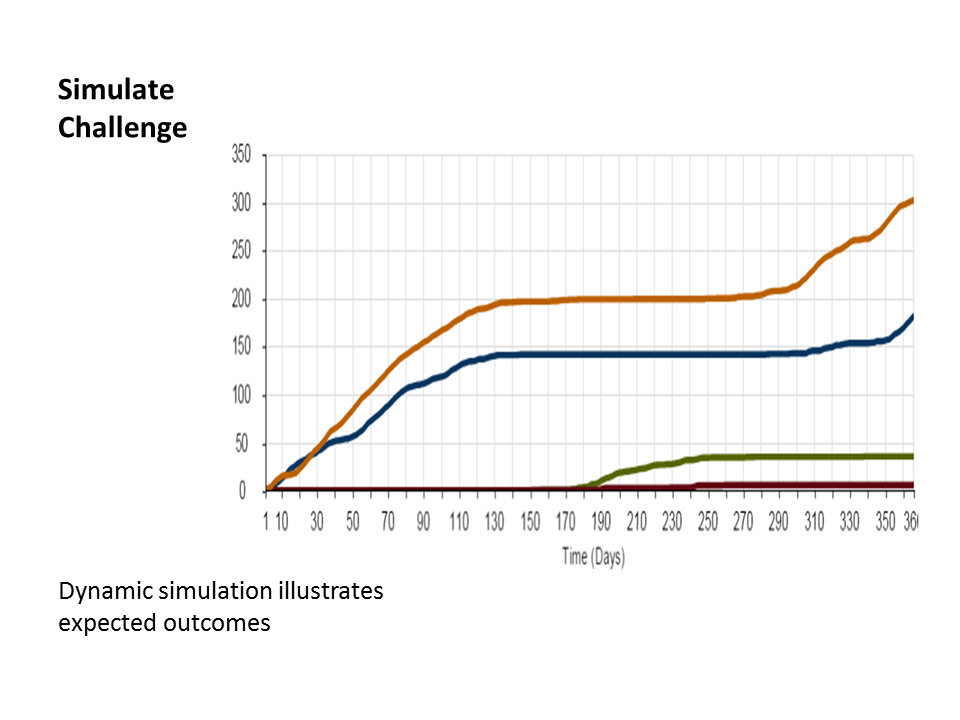
\includegraphics{img/cem5.png}
\caption[Systems Modelling and Visualisation]{Systems models can also be used to visualise the dynamics of the challenge. In our case we looked at daily excess mortality over a `typical year' in 2030 (climate change scenario) and a `typical year' in 2010s (control). We show excess cold stress mortality now (orange line) and in 2030 (blue line); we also illustrate heat stress mortality now (red line) and in the future (green line). Stakeholders can watch the simulation unfold. They can change the assumptions underlying the model including age range, SES and sex of the population. Furthermore, public health interventions can be `gamed' using the reach, compliance and efficacy expectations. Systems thinking and systems modelling provides a number of visual tools and dynamic simulations with which to engage and develop shared understanding of complex public health challenges. Although we have only begun to use these tools and explore their potential to engage, we can already see that compared with the usual lengthy reports, tabulated data, statistical models and significance values that public health professionals traditionally use to convey their `evidence base' for decision making.}
\end{figure}

\begin{figure}[htbp]
\centering
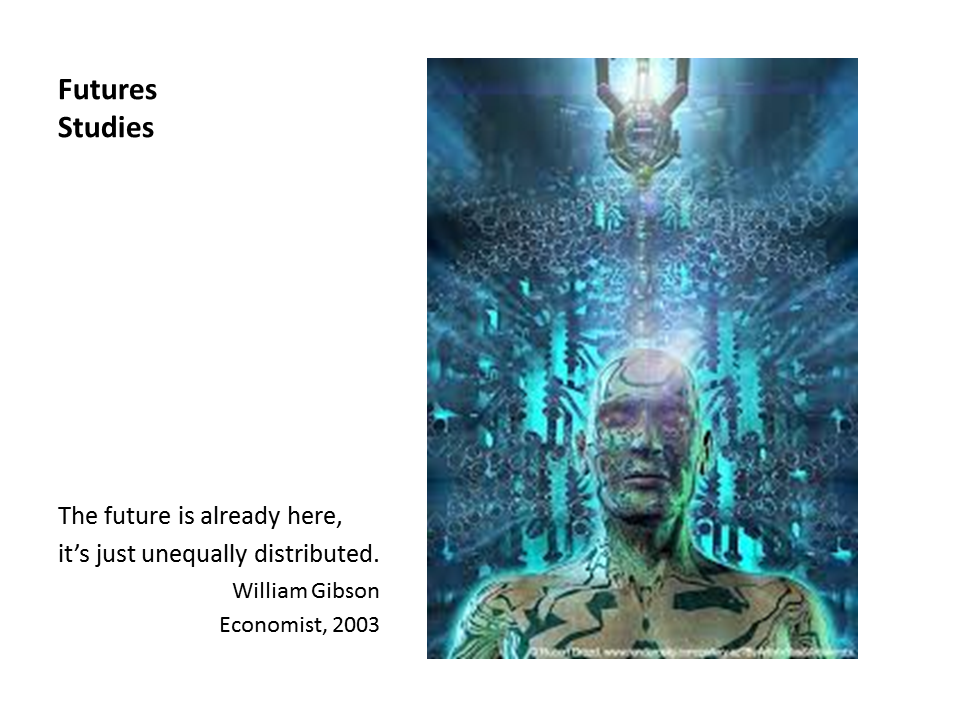
\includegraphics{img/cem6.png}
\caption[Futures Studies]{In addition to Systems Thinking -- the ``futures studies'' approach, encapsulated in this quote from William Gibson, promotes a large number of techniques that provide a basis upon which to extrapolate trends into the future for the purpose of describing the `future states' that are possible -- with the often stated aim of `shaping' strategy to aim for ``desirable future states''.
}
\end{figure}

\begin{figure}[htbp]
\centering
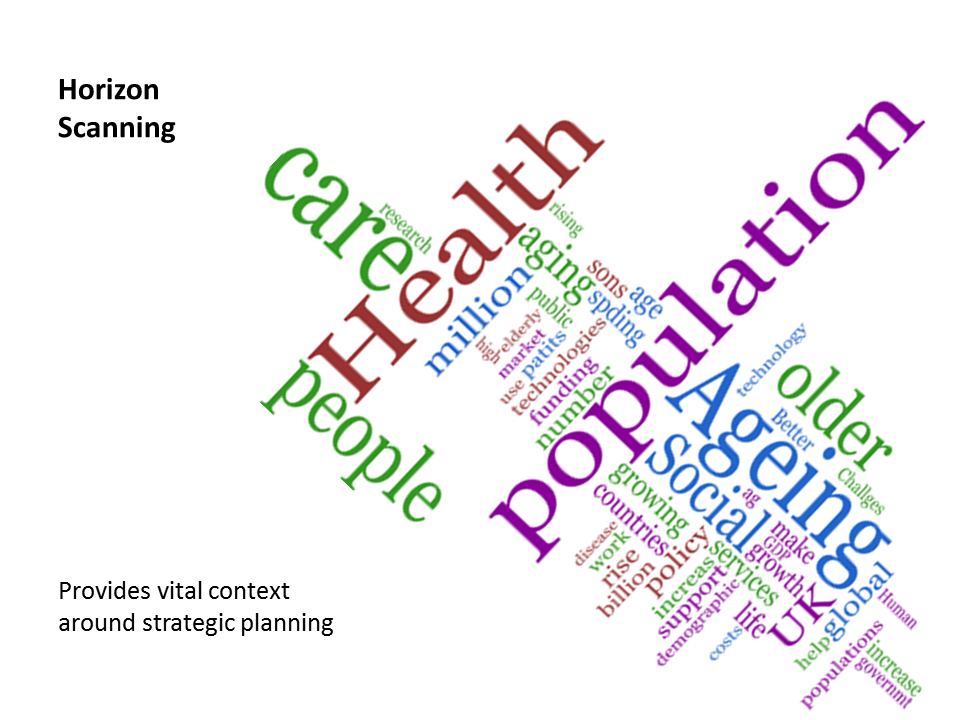
\includegraphics{img/cem7.png}
\caption[Horizon Scanning Method]{The first techniques we looked at is a fundamental tool in futures studies -- horizon scanning. It is almost a `reverse literature review' looking not at what has happened, but rather at what is likely to happen. The `grist' for horizon scanning is often not found in the peer-reviewed literature, but rather in industry reports, popular science magazines, government reviews and other sources that examine contemporary `trends'. Extrapolating trends leads to `scenario development', which explores the status of multiple trends at one or more fixed points in the future. Allowing for the description of a `future state' or future scenario.
}
\end{figure}

\begin{figure}[htbp]
\centering
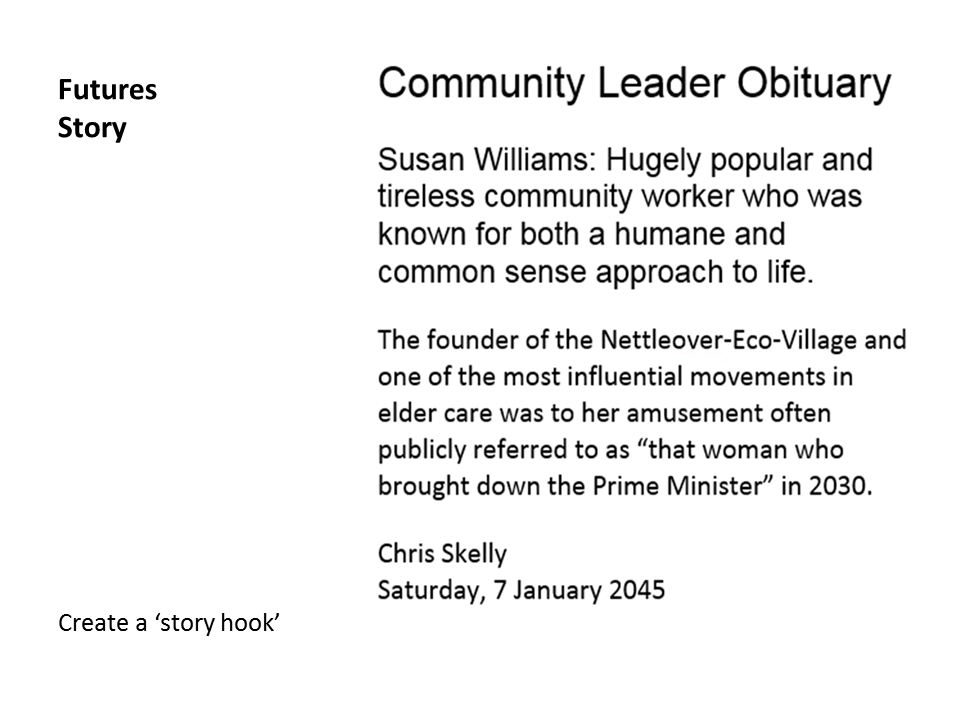
\includegraphics{img/cem8.png}
\caption[Futures Story Method]{Based upon the description of future scenarios that result from a horizon scanning exercise, a futures story is a short fictional story resting on a skeletal future scenario. The purpose of the futures story is to engage the reader. It is not primarily to inform, although this is a co-benefit. The purpose to `hook the reader' -- to engage in the telling of a story. The engaged reader might then be inclined to learn more -- to follow up the story using an online link explaining the future scenario and the trends that support its description.
}
\end{figure}

\begin{figure}[htbp]
\centering
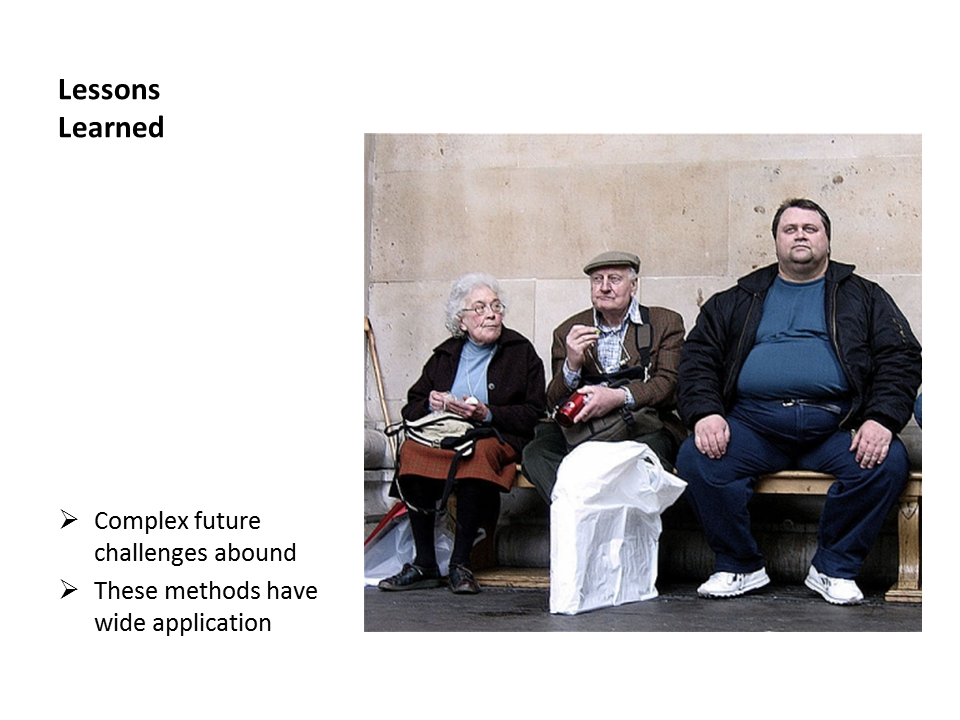
\includegraphics{img/cem9.png}
\caption[Understanding and Communicating Complexity]{Although this research did not start out to focus on approaches to meaningful engagement in complex public health challenges that is where it ended up. More over it is not an end, but rather, we believe, the beginning of a better approach to the contemporary complexity found in most public health challenges.}
\end{figure}

